\chapter{Plan de Trabajo}
\label{cap:plan}

Esta sección presenta el plan de trabajo del proyecto. La planificación se organiza en dos etapas que abarcan dos semestres. La primera corresponde al Seminario de Título (segundo semestre 2026), que incluye la planificación de la investigación, el desarrollo del Estado del Arte y la propuesta preliminar. La segunda etapa corresponde al Proyecto de Título (primer semestre 2027), donde se desarrolla e implementa la propuesta de solución, se ejecutan los experimentos y se redacta el informe final.

\section{Carta Gantt}
La figura \ref{fig:gantt1} presenta el cronograma integrado del segundo semestre 2026. En el cual se inicia Seminario de Título, con foco en el desarrollo de la metodología, Estado del Arte y propuesta de solución a nivel de componentes y las características de este.

\begin{figure}[htbp]
    \centering
    \makebox[\textwidth][c]{%
        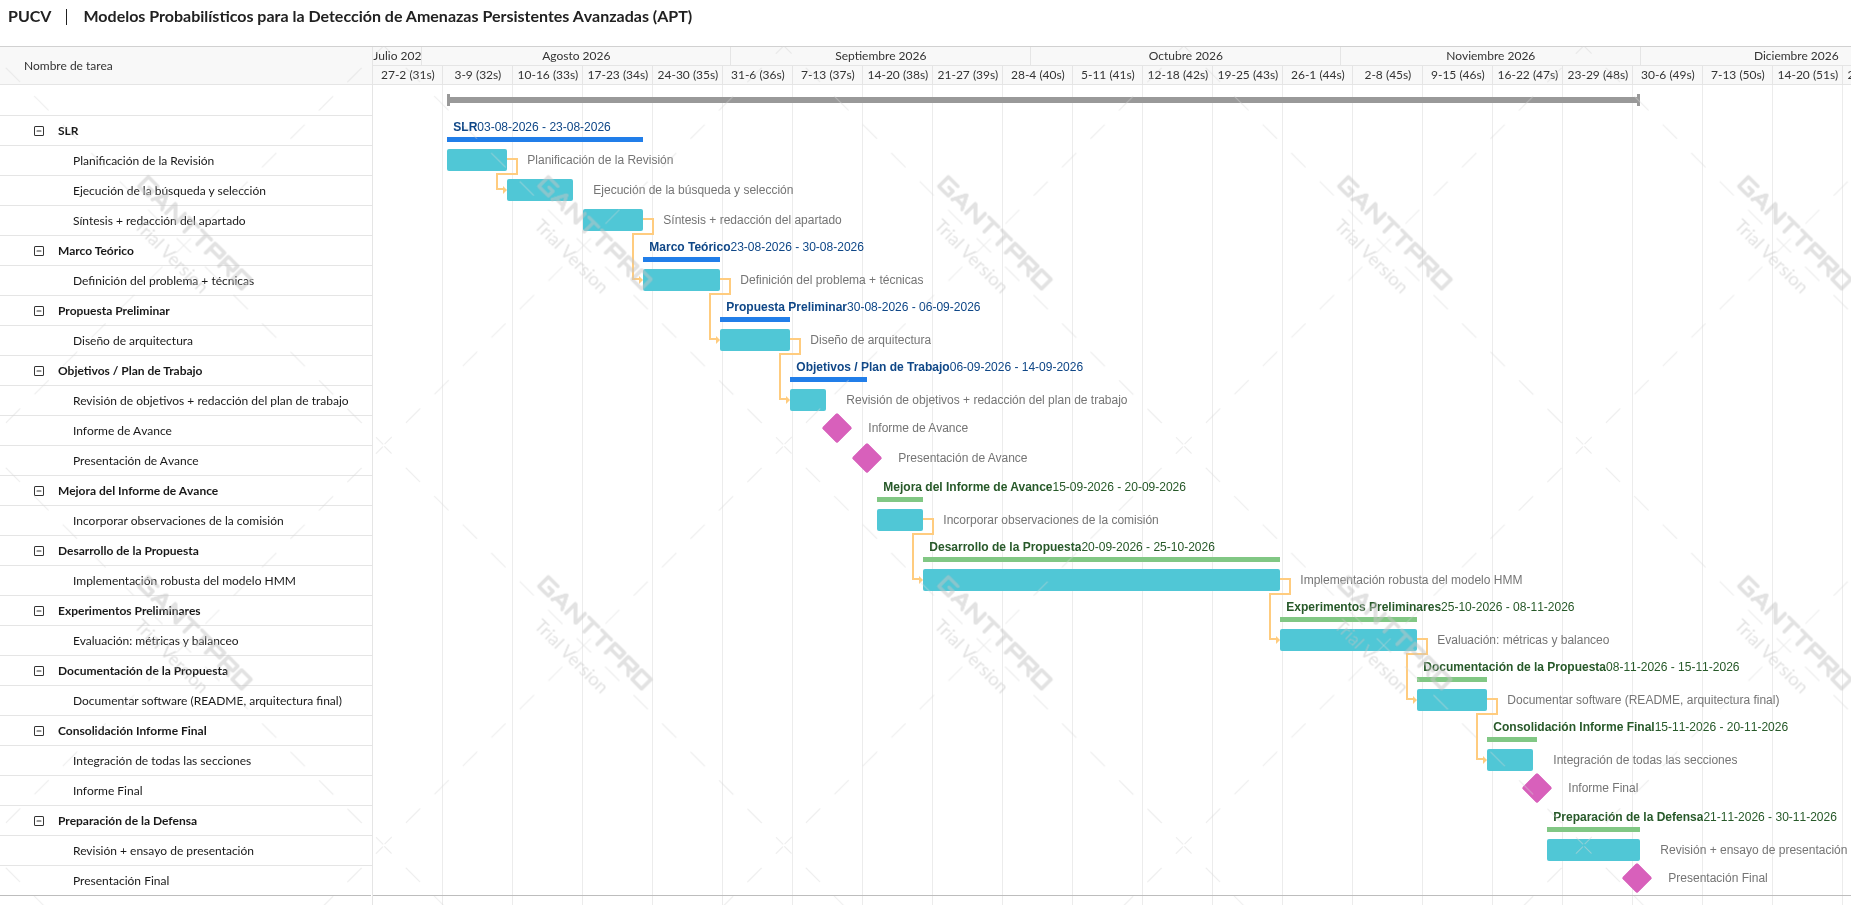
\includegraphics[width=0.95\paperwidth]{assets/CartaGantt1.png}%
    }
    \caption{Cronograma de actividades del Seminario de Título (agosto a noviembre de 2026). Fuente: Elaboración propia.}
    \label{fig:gantt1}
\end{figure}

\clearpage
\noindent
La Figura~\ref{fig:gantt2} presenta una planificación tentativa del primer semestre 2027, correspondiente a Proyecto de Título, con foco en el desarrollo e implementación completa de la propuesta de solución, las pruebas del sistema, la obtención de métricas de validación y la redacción del informe definitivo con los análisis de los resultados obtenidos. Dado que el calendario académico de dicho periodo aún no ha sido publicado, las fechas presentadas corresponden a estimaciones basadas en la duración habitual de un semestre y quedan sujetas a ajuste una vez que la Escuela fije las instancias formales de evaluación.

\vspace{0.5cm}

\begin{center}
    \makebox[\textwidth][c]{%
        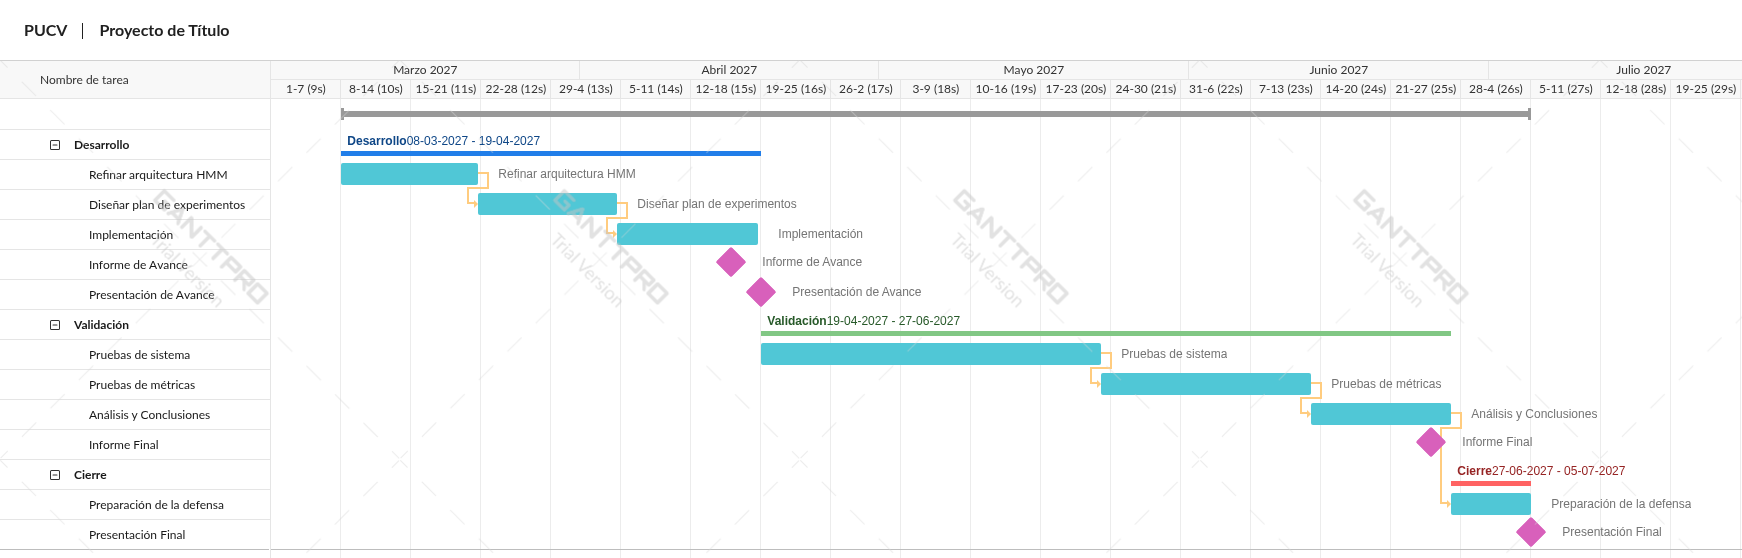
\includegraphics[width=0.95\paperwidth]{assets/CartaGantt2.png}%
    }
    \vspace{0.3cm}
    \captionof{figure}{Cronograma de actividades del Proyecto de Título (marzo a julio de 2027). Fuente: Elaboración propia.}
    \label{fig:gantt2}
\end{center}
